 
\chapter{Weighted Least Squares}\label{chapter::WLS}
 
\section{Generalized least squares}\label{section::GLS}

We can extend the Gauss--Markov model to allow for a general covariance
structure of the error term. The following model is due to \citet{aitkin1936least}.


\begin{assumption}
[Generalized Gauss--Markov model]
\label{assume::g-gaussmarkov}
We have 
\begin{eqnarray}
\label{eq::gls-model}
Y=X\beta+\varepsilon, \quad E(\varepsilon) = 0,\quad \cov(\varepsilon) = \sigma^2 \Sigma.
\end{eqnarray}
where $X$ is a fixed matrix with linearly independent columns.
The unknown parameters are  $\beta $ and $ \sigma^{2}$.
The $\Sigma$ is a known positive definite matrix.
\end{assumption}






Two leading cases of generalized least squares are
\begin{eqnarray}
\label{eq::diagonal-sigma}
\Sigma=\text{diag}\left\{ w_{1}^{-1},\ldots,w_{n}^{-1}\right\} ,
\end{eqnarray}
which corresponds to  a diagonal
covariance matrix, and 
\begin{eqnarray}
\label{eq::block-diagonal-sigma}
\Sigma = \text{diag}\left\{ \Sigma_1,\ldots, \Sigma_K\right\}
\end{eqnarray}
which corresponds to a block diagonal covariance matrix where $\Sigma_k$ is $n_k\times n_k$ and $\sum_{k=1}^K n_k = n$. 

Under model \eqref{eq::gls-model}, we can still use the OLS estimator $\hat{\beta}=(X^{\T}X)^{-1}X^{\T}Y$. It is unbiased 
$$
E(\hat{\beta}) = (X^{\T}X)^{-1}X^{\T}E(Y) = (X^{\T}X)^{-1}X^{\T} X\beta = \beta . 
$$
It has covariance matrix
\begin{align}
\cov(\hat{\beta}) & =\cov\left\{ (X^{\T}X)^{-1}X^{\T}Y\right\} \nonumber \\
 & =(X^{\T}X)^{-1}X^{\T}\cov(Y)X(X^{\T}X)^{-1}\nonumber \\
 & =\sigma^{2}(X^{\T}X)^{-1}X^{\T}\Sigma X(X^{\T}X)^{-1}.\label{eq:cov-ols-generalmodel}
\end{align}
The OLS estimator is BLUE under the Gauss--Markov model, but it is
not under the generalized Gauss--Markov model. Then what is the BLUE? We can transform \eqref{eq::gls-model} into the Gauss--Markov model by standardizing the error
term: 
\[
\Sigma^{-1/2}Y=\Sigma^{-1/2}X\beta+\Sigma^{-1/2}\varepsilon.
\]
Define $Y_* =\Sigma^{-1/2}Y, X_*=\Sigma^{-1/2}X$ and $ \varepsilon_* =\Sigma^{-1/2}\varepsilon$.
The model \eqref{eq::gls-model} reduces to 
\[
Y_* =\tilde{X}\beta+ \varepsilon_*,\quad E(\varepsilon_*) = 0, \quad \cov(\varepsilon_*) = \sigma^{2}I_{n},
\]
which is the Gauss--Markov model for the transformed variables  $Y_*$ and $X_*$. 
The Gauss--Markov theorem ensures that the BLUE is
\[
\hat{\beta}_{\Sigma}=({X}_*^{\T}{X}_*)^{-1}{X}_*^{\T}{Y}_*=(X^{\T}\Sigma^{-1}X)^{-1}X^{\T}\Sigma^{-1}Y . 
\]
It is unbiased because
\begin{eqnarray*}
E(\hat{\beta}_{\Sigma}) 
&=& (X^{\T}\Sigma^{-1}X)^{-1}X^{\T}\Sigma^{-1}E(Y) \\
&=& (X^{\T}\Sigma^{-1}X)^{-1}X^{\T}\Sigma^{-1}X\beta \\
&=&\beta . 
\end{eqnarray*}
It has covariance matrix
\begin{align}
\cov(\hat{\beta}_{\Sigma}) & =\cov\left\{ (X^{\T}\Sigma^{-1}X)^{-1}X^{\T}\Sigma^{-1}Y\right\} \nonumber \\
 & =(X^{\T}\Sigma^{-1}X)^{-1}X^{\T}\Sigma^{-1}\cov(Y)\Sigma^{-1}X(X^{\T}\Sigma^{-1}X)^{-1}\nonumber \\
 & =\sigma^{2}(X^{\T}\Sigma^{-1}X)^{-1}X^{\T}\Sigma^{-1}\Sigma\Sigma^{-1}X(X^{\T}\Sigma^{-1}X)^{-1}\nonumber \\
 & =\sigma^{2}(X^{\T}\Sigma^{-1}X)^{-1}.\label{eq:cov-wls-generalmodel}
\end{align}
In particular, $\cov(\hat{\beta}_{\Sigma})$ is
smaller than or equal to $\cov(\hat{\beta})$ in the matrix sense\footnote{The matrix $X^{\T}\Sigma^{-1} X$ is positive definite and thus invertible,
because (1) for any $\alpha\in\mathbb{R}^{p}$, 
\[
\Sigma^{-1} \succeq0\Longrightarrow\alpha^{\T}X^{\T}\Sigma X\alpha\geq0,
\]
and (2) 
$$
\alpha^{\T}X^{\T}\Sigma X\alpha  =0\Longleftrightarrow X\alpha=0
  \Longleftrightarrow\alpha=0
$$
since $X$ has linearly independent columns. }. 
%The Gauss--Markov theorem ensures that 
%\[
%\cov(\hat{\beta}_{\Sigma})\preceq\cov(\hat{\beta}),
%\]
%which, coupled with 
So based on
(\ref{eq:cov-ols-generalmodel}) and (\ref{eq:cov-wls-generalmodel}),
we have the following pure linear algebra inequality:
\begin{corollary}\label{corollary::WLS-linear-algebra}
If $X$ has linear independent columns and $\Sigma$ is invertible, then 
\[
(X^{\T}\Sigma^{-1}X)^{-1}\preceq(X^{\T}X)^{-1}X^{\T}\Sigma X(X^{\T}X)^{-1}.
\]
\end{corollary}

Problem \ref{hw16::linear-algebra-wls} gives a more general result. 


\section{Weighted least squares}


This chapter focuses on the first covariance structure in \eqref{eq::diagonal-sigma} and Chapter \ref{chapter::gee} will discuss the second in \eqref{eq::block-diagonal-sigma}.  The $\Sigma$ in \eqref{eq::diagonal-sigma} results in the weighted least squares (WLS) estimator
\begin{eqnarray*}
\hat{\beta}_{w}  =\hat{\beta}_{\Sigma}
&=& (X^{\T}\Sigma^{-1}X)^{-1}X^{\T}\Sigma^{-1}Y \\
&=&\left(\sumn w_{i}x_{i}x_{i}^{\T}\right)^{-1}\sumn w_{i}x_{i}y_{i}.
\end{eqnarray*}
From the derivation above, we can also write the WLS estimator as
\begin{align*}
\hat{\beta}_{w}  
 & =\arg\min_{b\in \mathbb{R}^p}(Y-Xb)^{\T}\Sigma^{-1}(Y-Xb) \\
&  =\arg\min_{b\in \mathbb{R}^p}\sumn w_{i}(y_{i}-x_{i}^{\T}b)^{2}\\
  &=\arg\min_{b\in \mathbb{R}^p}( Y_*  - X_*  b)^{\T} ( Y_* -  X_* b)  \\
&  =\arg\min_{b\in \mathbb{R}^p}\sumn( y_{*i}  -x_{*i}^{\T} b)^{2},
\end{align*}
where $y_{*i} =w_{i}^{1/2}y_{i}$ and $x_{*i} =w_{i}^{1/2}x_{i}$. So
WLS is equivalent to the OLS with transformed variables, with the weights inversely proportional to the variances of the errors. 
By this equivalence, WLS inherits many properties of OLS. See the problems in Section \ref{sec::homework-problems} for more details. 



%\section{Statistical inference with WLS}
%I will discuss statistical inference with the WLS estimator $\hat{\beta}_{w}$. 

Analogous to OLS, we can derive finite-sample exact inference based on the generalized Normal linear model:
$$
y_{i}=x_{i}^{\T}\beta+\varepsilon_{i},\quad \varepsilon_{i} \sim \N(0, \sigma^2/w_i),
$$
or, equivalently,
$$
y_{*i} = x_{*i}^{\T}\beta+ \varepsilon_{*i},\quad \varepsilon_{*i} \sim \N(0, \sigma^2).
$$
%where $\tilde{y}_{i}  = w_i^{1/2} y_i$ and $\tilde{x}_i = w_i^{1/2} x_i$. 
The \ri{lm} function with \ri{weights} reports the standard error, $t$-statistic, and $p$-value based on this model. This assumes that the weights fully capture the heteroskedasticity, which is unrealistic in many problems. 

In addition, we can derive asymptotic inference based on the following heteroskedastic model
\[
y_{i}=x_{i}^{\T}\beta+\varepsilon_{i}
\]
where the $\varepsilon_{i}$'s are independent with mean zero and
variances $\sigma_{i}^{2}\ (i=1,\ldots,n)$. It is possible that $w_{i}\neq1/\sigma_{i}^{2}$,
i.e., the variances used to construct the WLS estimator can be misspecified.
Even though there is no guarantee that $\hat{\beta}_{w}$ is BLUE,
it is still unbiased. From the decomposition
\begin{align*}
\hat{\beta}_{w} & =\left(\sumn w_{i}x_{i}x_{i}^{\T}\right)^{-1}\sumn w_{i}x_{i}y_{i}\\
 & =\left(\sumn w_{i}x_{i}x_{i}^{\T}\right)^{-1}\sumn w_{i}x_{i}(x_{i}^{\T}\beta+\varepsilon_{i})\\
 & =\beta+\left(n^{-1}\sumn w_{i}x_{i}x_{i}^{\T}\right)^{-1}\left(n^{-1}\sumn w_{i}x_{i}\varepsilon_{i}\right),
\end{align*}
we can apply the law of large numbers to show that $\hat{\beta}_{w}$
is consistent for $\beta$ and apply the CLT to
show that 
\[
\hat{\beta}_{w}\asim\N\left(\beta,V_w\right),
\]
where 
\[
V_w  = n^{-1}\left(n^{-1}\sumn w_{i}x_{i}x_{i}^{\T}\right)^{-1}\left(n^{-1}\sumn w_{i}^{2}\sigma_{i}^{2}x_{i}x_{i}^{\T}\right)\left(n^{-1}\sumn w_{i}x_{i}x_{i}^{\T}\right)^{-1}. 
\]
The EHW robust covariance generalizes to
\[
\hat{V}_{\ehw, w}=n^{-1}\left(n^{-1}\sumn w_{i}x_{i}x_{i}^{\T}\right)^{-1}\left(n^{-1}\sumn w_{i}^{2}\hat{\varepsilon}_{w,i}^{2}x_{i}x_{i}^{\T}\right)\left(n^{-1}\sumn w_{i}x_{i}x_{i}^{\T}\right)^{-1},
\]
where $\hat{\varepsilon}_{w,i}=y_{i}-x_{i}^{\T}\hat{\beta}_{w}$ is
the residual from the WLS. Note that in the sandwich covariance, $w_{i}$
appears in the ``bread'' but $w_{i}^{2}$ appears in the ``meat.'' This formula appeared in \citet{magee1998improving} and \citet{romano2017resurrecting}. The  function
\ri{hccm} in the 
\ri{R} package \ri{car} can compute various EHW covariance estimators based on WLS. To save space in the examples below, I report only the standard errors based on the generalized Normal linear model and leave the calculations of the EHW covariances as a homework problem. 





\section{WLS motivated by heteroskedasticity}

%An important practical question is: where do these weights come from?
%The first two cases below have weights motivated by heteroskedasticity,
%and the last two cases are motivated by issues beyond heteroskedasticity. 

\subsection{Feasible generalized least squares}\label{section::fgls}

Assume that $\varepsilon$ has mean zero and covariance $\text{diag}\left\{ \sigma_{1}^{2},\ldots,\sigma_{n}^{2}\right\} $.
If the $\sigma_{i}^{2}$'s are known, we can simply apply the WLS
above; if they are unknown, we need to estimate them first. This gives
the following feasible generalized least squares estimator (FGLS):
\begin{enumerate}
\item Run OLS of $y_i$ on $x_i$ to obtain the residuals $\hat{\varepsilon}_i$. Then obtain the squared residuals $\hat{\varepsilon}_i^2.$

\item \label{enu:fgls-step2}Run OLS of $\log(\hat{\varepsilon}^{2}_i)$ on
$x_i$ to obtain the fitted values and exponentiate them to obtain $(\hat{\sigma}_{i}^{2})_{i=1}^{n}$;
\item Run WLS of $y_i$ on $x_i$ with weights $ \hat{\sigma}_{i}^{-2} $
to obtain
\[
\hat{\beta}_{\textsc{fgls}}=\left(\sumn\hat{\sigma}_{i}^{-2}x_{i}x_{i}^{\T}\right)^{-1}\sumn\hat{\sigma}_{i}^{-2}x_{i}y_{i}.
\]
\end{enumerate}
%
In Step \ref{enu:fgls-step2}, we can change the model based
on our understanding of heteroskedasticity. Here I use the Boston housing data to compare the OLS and FGLS, with \ri{R} code in \ri{code18.3.1.R}.

\begin{lstlisting}
> library(mlbench)
> data(BostonHousing)
> ols.fit = lm(medv ~ ., data = BostonHousing)
> dat.res = BostonHousing
> dat.res$medv = log((ols.fit$residuals)^2)
> t.res.ols = lm(medv ~ ., data = dat.res)
> w.fgls = exp(-t.res.ols$fitted.values)
> fgls.fit = lm(medv ~ ., weights = w.fgls, data = BostonHousing)
> ols.fgls = cbind(summary(ols.fit)$coef[,1:3], 
+                  summary(fgls.fit)$coef[,1:3])
> round(ols.fgls, 3)
            Estimate Std. Error t value Estimate Std. Error t value
(Intercept)   36.459      5.103   7.144    9.499      4.064    2.34
crim          -0.108      0.033  -3.287   -0.081      0.044   -1.82
zn             0.046      0.014   3.382    0.030      0.011    2.67
indus          0.021      0.061   0.334   -0.035      0.038   -0.92
chas1          2.687      0.862   3.118    1.462      1.119    1.31
nox          -17.767      3.820  -4.651   -7.161      2.784   -2.57
rm             3.810      0.418   9.116    5.675      0.364   15.59
age            0.001      0.013   0.052   -0.044      0.008   -5.50
dis           -1.476      0.199  -7.398   -0.927      0.139   -6.68
rad            0.306      0.066   4.613    0.170      0.051    3.31
tax           -0.012      0.004  -3.280   -0.010      0.002   -4.14
ptratio       -0.953      0.131  -7.283   -0.700      0.094   -7.45
b              0.009      0.003   3.467    0.014      0.002    6.54
lstat         -0.525      0.051 -10.347   -0.158      0.036   -4.38
\end{lstlisting}

Unfortunately, the coefficients, including the point estimates and standard errors, from OLS and FGLS are quite different for several covariates. This suggests that the linear model may be misspecified. Otherwise, both estimators are consistent for the same true coefficient, and they should not be so different even in the presence of randomness. 



The above FGLS estimator is close to \citet[][Chapter 8]{wooldridge2012introductory}. \citet{romano2017resurrecting} propose to regress $\log ( \max(\delta^2, \hat \varepsilon_i^2) )$ on $ \log | x_{i1} |, \ldots, \log  |x_{ip}|$ to estimate the individual variances. Their modification has two features: first, they truncate the small residuals by a pre-specified positive number $\delta^2$; second, their regressors are the logs of the absolute values of the original covariates. 
\citet{romano2017resurrecting} highlighted the efficiency gain from the FGLS compared to OLS in the presence of heteroskedasticity. 
\citet{diciccio2019improving} proposed some improved versions of the FGLS estimator even if the variance function is misspecified. However, it is unusual for practitioners to use FGLS even though it can be more efficient than OLS. There are several reasons. First, the EHW standard errors are convenient for correcting the standard error of OLS under heteroskedasticity. Second, the efficiency gain is usually small, and it is even possible that the FGLS is less efficient than OLS when the variance function is misspecified. Third, the linear model is very likely to be misspecified, and if so, OLS and FGLS estimate different parameters. The OLS has the interpretations as the best linear predictor and the best linear approximation of the conditional mean, but the FGLS has more complicated interpretations when the linear model is wrong. Based on these reasons, we need to carefully justify the choice of FGLS  over  OLS in real data analyses. 
 


\subsection{Aggregated data and ecological regression}
\label{sec::regression-aggregateddata}


%\subsubsection{WLS with aggregated data}

In some case, $(y_{i},x_{i})$ come from aggregated data, for example,
$y_{i}$ can be the average test score and $x_{i}$ can be the average
parents' income of students within classroom $i$. If we believe that
the student-level test score and parents' income follow a homoskedastic
linear model, then the model based on the classroom average must be
heteroskedastic, with the variance inversely proportional to the
classroom size. In this case, a natural choice of weight is $w_{i}=n_{i}$,
the classroom size. 



\begin{figure}
\centering
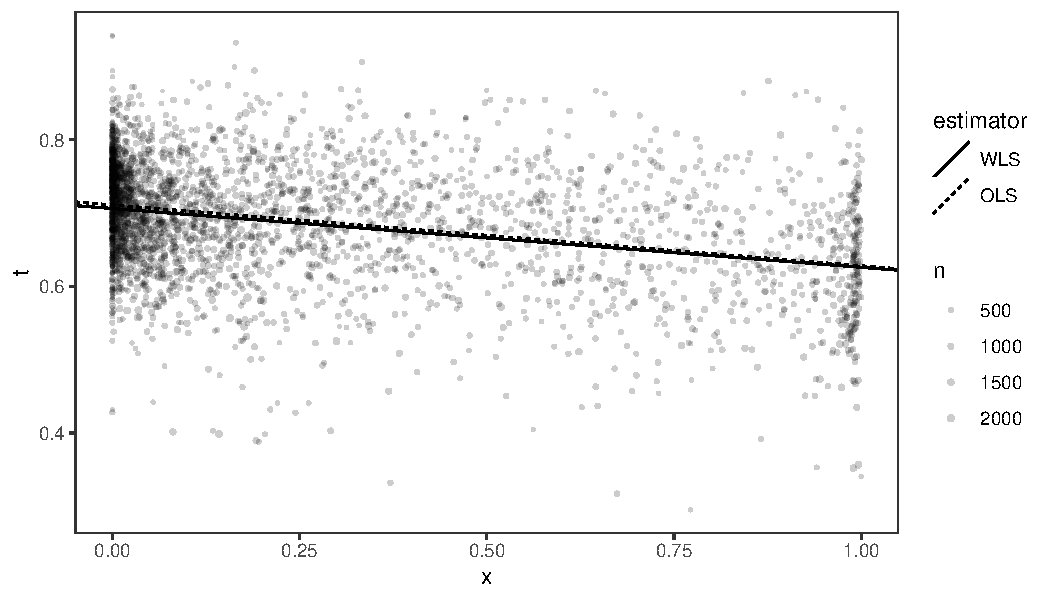
\includegraphics[width = \textwidth]{figures/lavoteall_plot.pdf}
\caption{Fulton data}\label{fig::lavoteall}
\end{figure}




Below I use the  \ri{lavoteall} dataset from the \ri{R} package \ri{ei}. It contains the 
the fraction of black registered voters \ri{x}, the fraction of voter turnout \ri{t}, and the total number of people \ri{n} in each Louisiana precinct. 
Figure \ref{fig::lavoteall} is the scatterplot. In this example, OLS and WLS give similar results although \ri{n} varies a lot across precincts. 


\begin{lstlisting}
> library("ei")
> data(lavoteall)
> ols.fit = lm(t ~ x, data = lavoteall)
> wls.fit = lm(t ~ x, weights = n, data = lavoteall)
> compare = cbind(summary(ols.fit)$coef[,1:3], 
+                 summary(wls.fit)$coef[,1:3])
> round(compare, 3)
            Estimate Std. Error t value Estimate Std. Error t value
(Intercept)    0.711      0.002 408.211    0.706      0.002 421.662
x             -0.083      0.004 -19.953   -0.080      0.004 -19.938
\end{lstlisting}




 
In the above, we can interpret the coefficient of \ri{x} as the precinct-level relationship between the fraction of black registered voters and the fraction voting. Political scientists are interested in using aggregated data to infer individual voting behavior.
Hypothetically, the precinct $i$ has individual data $\{  x_{ij}, y_{ij}  : j = 1, \ldots, n_i\}$ where $x_{ij}$ and $y_{ij}$ are the binary racial and voting status of individual $(i, j)$ $(i=1,\ldots, n; j = 1, \ldots, n_i)$. However, we only observe the aggregated data $\{ \bar{x}_{i\cdot}, \bar{y}_{i\cdot}, n_i :  i = 1,\ldots, n\}$, where 
$$
\bar{x}_{i\cdot} = n_i^{-1} \sum_{j=1}^{n_i}  x_{ij},\quad
\bar{y}_{i\cdot} = n_i^{-1} \sum_{j=1}^{n_i}  y_{ij}
$$ 
are the fraction of black registered voters and the fraction voting, respectively. Can we infer the individual voting behavior based on the aggregated data? In general, this is almost impossible. Under some assumptions, we can make progress. Goodman's ecological regression below is one possibility.  


Assume that for precinct $i = 1,\ldots, n$, we have
$$
y_{ij} \mid x_{ij} = 1 \iidsim \text{Bernoulli}(p_{i1}),\quad
y_{ij} \mid x_{ij} = 0 \iidsim \text{Bernoulli}(p_{i0}),\quad 
(j = 1, \ldots, n_i) . 
$$
This is the individual-level model, where the $p_{i1}$'s and $p_{i0}$'s measure the association between race and voting.
We further assume that they are random and independent of the $x_{ij}$'s, with means
\begin{equation}\label{eq::ecological-assumption-1}
E( p_{i1} ) = p_1,\quad
E( p_{i0} ) = p_0.
\end{equation}
Then we can decompose the aggregated outcome variable as 
\begin{eqnarray*}
\bar{y}_{i\cdot} &=&  n_i^{-1} \sum_{j=1}^{n_i}  y_{ij}  \\
&=&n_i^{-1} \sum_{j=1}^{n_i}   \{  x_{ij}  y_{ij}  + (1-x_{ij}) y_{ij}  \} \\
&=& n_i^{-1} \sum_{j=1}^{n_i}   \{  x_{ij}  p_{1}  + (1-x_{ij}) p_0  \}  + \varepsilon_i  \\
&=&  p_1 \bar{x}_{i\cdot}   + p_0 (1 -\bar{x}_{i\cdot} ) + \varepsilon_i,
\end{eqnarray*} 
where
$$
\varepsilon_i = n_i^{-1} \sum_{j=1}^{n_i}   \{  x_{ij}  (y_{ij} - p_{1} )   + (1-x_{ij}) ( y_{ij} -  p_0 ) \}.
$$
So we have a linear relationship between the aggregated outcome and covariate
$$
\bar{y}_{i\cdot}  = p_1 \bar{x}_{i\cdot}   + p_0 (1 -\bar{x}_{i\cdot} ) + \varepsilon_i,
$$
where 
$$
E(\varepsilon_i  \mid \bar{x}_{i\cdot}  ) = 0.
$$
\citet{goodman1953ecological} suggested to use the OLS of $\bar{y}_{i\cdot} $ on $\{ \bar{x}_{i\cdot}, (1 -\bar{x}_{i\cdot} )\}$ to estimate $(p_1, p_0)$, and \citet{goodman1959some} suggested to use the corresponding WLS with weight $n_i$ since the variance of $\varepsilon_i$ has the magnitude $n_i^{-1}$. Moreover, the variance of $\varepsilon_i$ has a rather complicated form of heteroskedasticity, so we should use the EHW standard error for inference. This is called Goodman's regression or ecological regression. The \ri{R} code in \ri{code18.3.2.R} implements ecological regression based on the \ri{lavoteall} data. 



\begin{lstlisting}
> ols.fit = lm(t ~ 0 + x + I(1-x), data = lavoteall)
> wls.fit = lm(t ~ 0 + x + I(1-x), weights = n, data = lavoteall)
> compare = cbind(summary(ols.fit)$coef[,1:3], 
+                 summary(wls.fit)$coef[,1:3])
> round(compare, 3)
         Estimate Std. Error t value Estimate Std. Error t value
x           0.628      0.003 188.292    0.626      0.003 194.493
I(1 - x)    0.711      0.002 408.211    0.706      0.002 421.662
\end{lstlisting}


The assumption in \eqref{eq::ecological-assumption-1} is crucial, which can be too strong when the precinct level $p_{i1}$'s and $p_{i0}$'s vary in systematic but unobserved ways. When the assumption is violated, it is possible that the ecological regression yields the opposite result compared to the individual regression. This is called the {\it ecological fallacy}. 

Another obvious problem of ecological regression is that the estimated coefficients may lie outside of the interval $[0,1]$. Problem \ref{hw16::ecological-regression2} gives an example. 

\citet{gelman2001models} gave an alternative set of assumptions justifying the ecological regression. \citet{king1997solution} proposed some extensions. \citet{robinson1950ecological}  warned that the ecological correlation might not inform individual correlation. \citet{freedman1991ecological} warned that the assumptions underlying the ecological regression might not be plausible in practice. 




\section{WLS with other motivations}

WLS can be used in other settings unrelated to heteroskedasticity. I review two examples below. 

\subsection{Local linear regression}

\begin{figure}
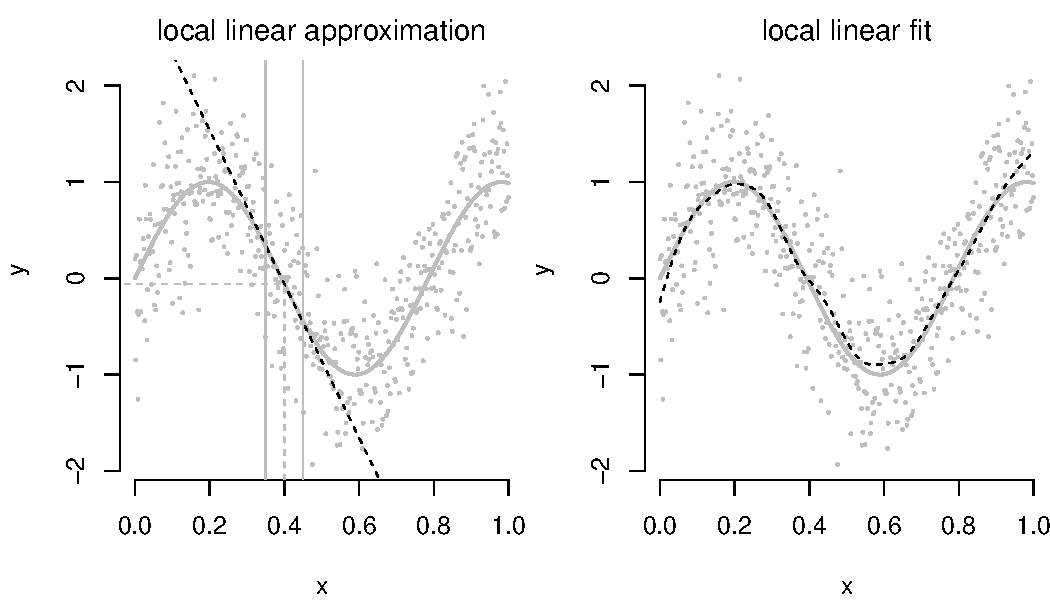
\includegraphics[width = \textwidth]{figures/localpolynomialplot}

\caption{Local linear regression}\label{fig::locallinearregression}
\end{figure}

Calculus tells us that locally we can approximate any smooth function $f(x)$
by a linear function even though the original function can be highly
nonlinear:
$$
f(x) \approx  f(x_0) + f'(x_0) (x - x_0) 
$$
when $x$ is near $x_0$. 
The left panel of Figure \ref{fig::locallinearregression} shows that in the neighborhood of $x_0=0.4$, even a sine function can be well approximated by a line. Based on data $(x_{i},y_{i})_{i=1}^{n}$, if we want to
predict the mean value of $y$ given $x=x_{0}$, then we can predict
based on a line with the local data points close to $x_{0}$.
It is also reasonable to down weight the points that are far from $x_{0}$,
which motivates the following WLS:
\[
(\hat{\alpha},\hat{\beta})=\arg\min_{a,b}\sumn w_{i}\left\{ y_{i}-a-b(x_{i}-x_{0})\right\} ^{2}
\]
with $w_{i}=K\left\{ (x_i -x_{0})/h\right\} $ where $K(\cdot)$ is called
the kernel function and $h$ is called the bandwidth parameter. With
the fitted line $\hat{y}(x)=\hat{\alpha}+\hat{\beta}(x-x_{0})$,
the predicted value at $x=x_{0}$ is the intercept $\hat{\alpha}$. 

Technically, $K(\cdot)$ can be any density function, and two canonical
choices are the standard Normal density and the Epanechikov kernel
$K(t)=0.75(1-t^{2})1(|t|\leq1).$ The choice of the kernel does not
matter that much. The choice of the bandwidth matters much more.
With large bandwidth, we have a poor linear approximation, leading to
bias; with small bandwidth, we have few data points, leading to large
variance. In practice, we face a bias-variance trade-off. In practice, we can either use cross-validation or other criterion to select $h.$


In general, we can approximate a smooth function by a polynomial:
$$
f(x) \approx  \sum_{k=0}^K  \frac{  f^{(k)}(x_0)  }{k!}  (x - x_0)^k 
$$
when $x$ is near $x_0$. So
we can even fit a polynomial function locally, which is called local polynomial regression \citep{fan1996local}. 
In the \ri{R} package \ri{Kernsmooth}, the function \ri{locpoly} fits local polynomial regression, and the function \ri{dpill} selects $h$ based on \citet{ruppert1995effective}. The default specification of \ri{locpoly}  is the local linear regression. 


\begin{lstlisting}
> library("KernSmooth")
> n = 500
> x = seq(0, 1, length.out = n)
> fx= sin(8*x)
> y = fx + rnorm(n, 0, 0.5)
> plot(y ~ x, pch = 19, cex = 0.2, col = "grey", bty = "n",
+      main = "local linear fit", font.main = 1)
> lines(fx ~ x, lwd = 2, col = "grey")
> h = dpill(x, y)
> locp.fit = locpoly(x, y, bandwidth = h)
> lines(locp.fit, lty = 2)
\end{lstlisting}



\subsection{Regression with survey data}
\label{sec::regression-surveydata}

Most discussions in this book are based on i.i.d. samples, or, at
least, the sample represents the population of interest. Sometimes, researchers over sample some units and under sample some other
units from a population of interest. 

\begin{figure}
\centering
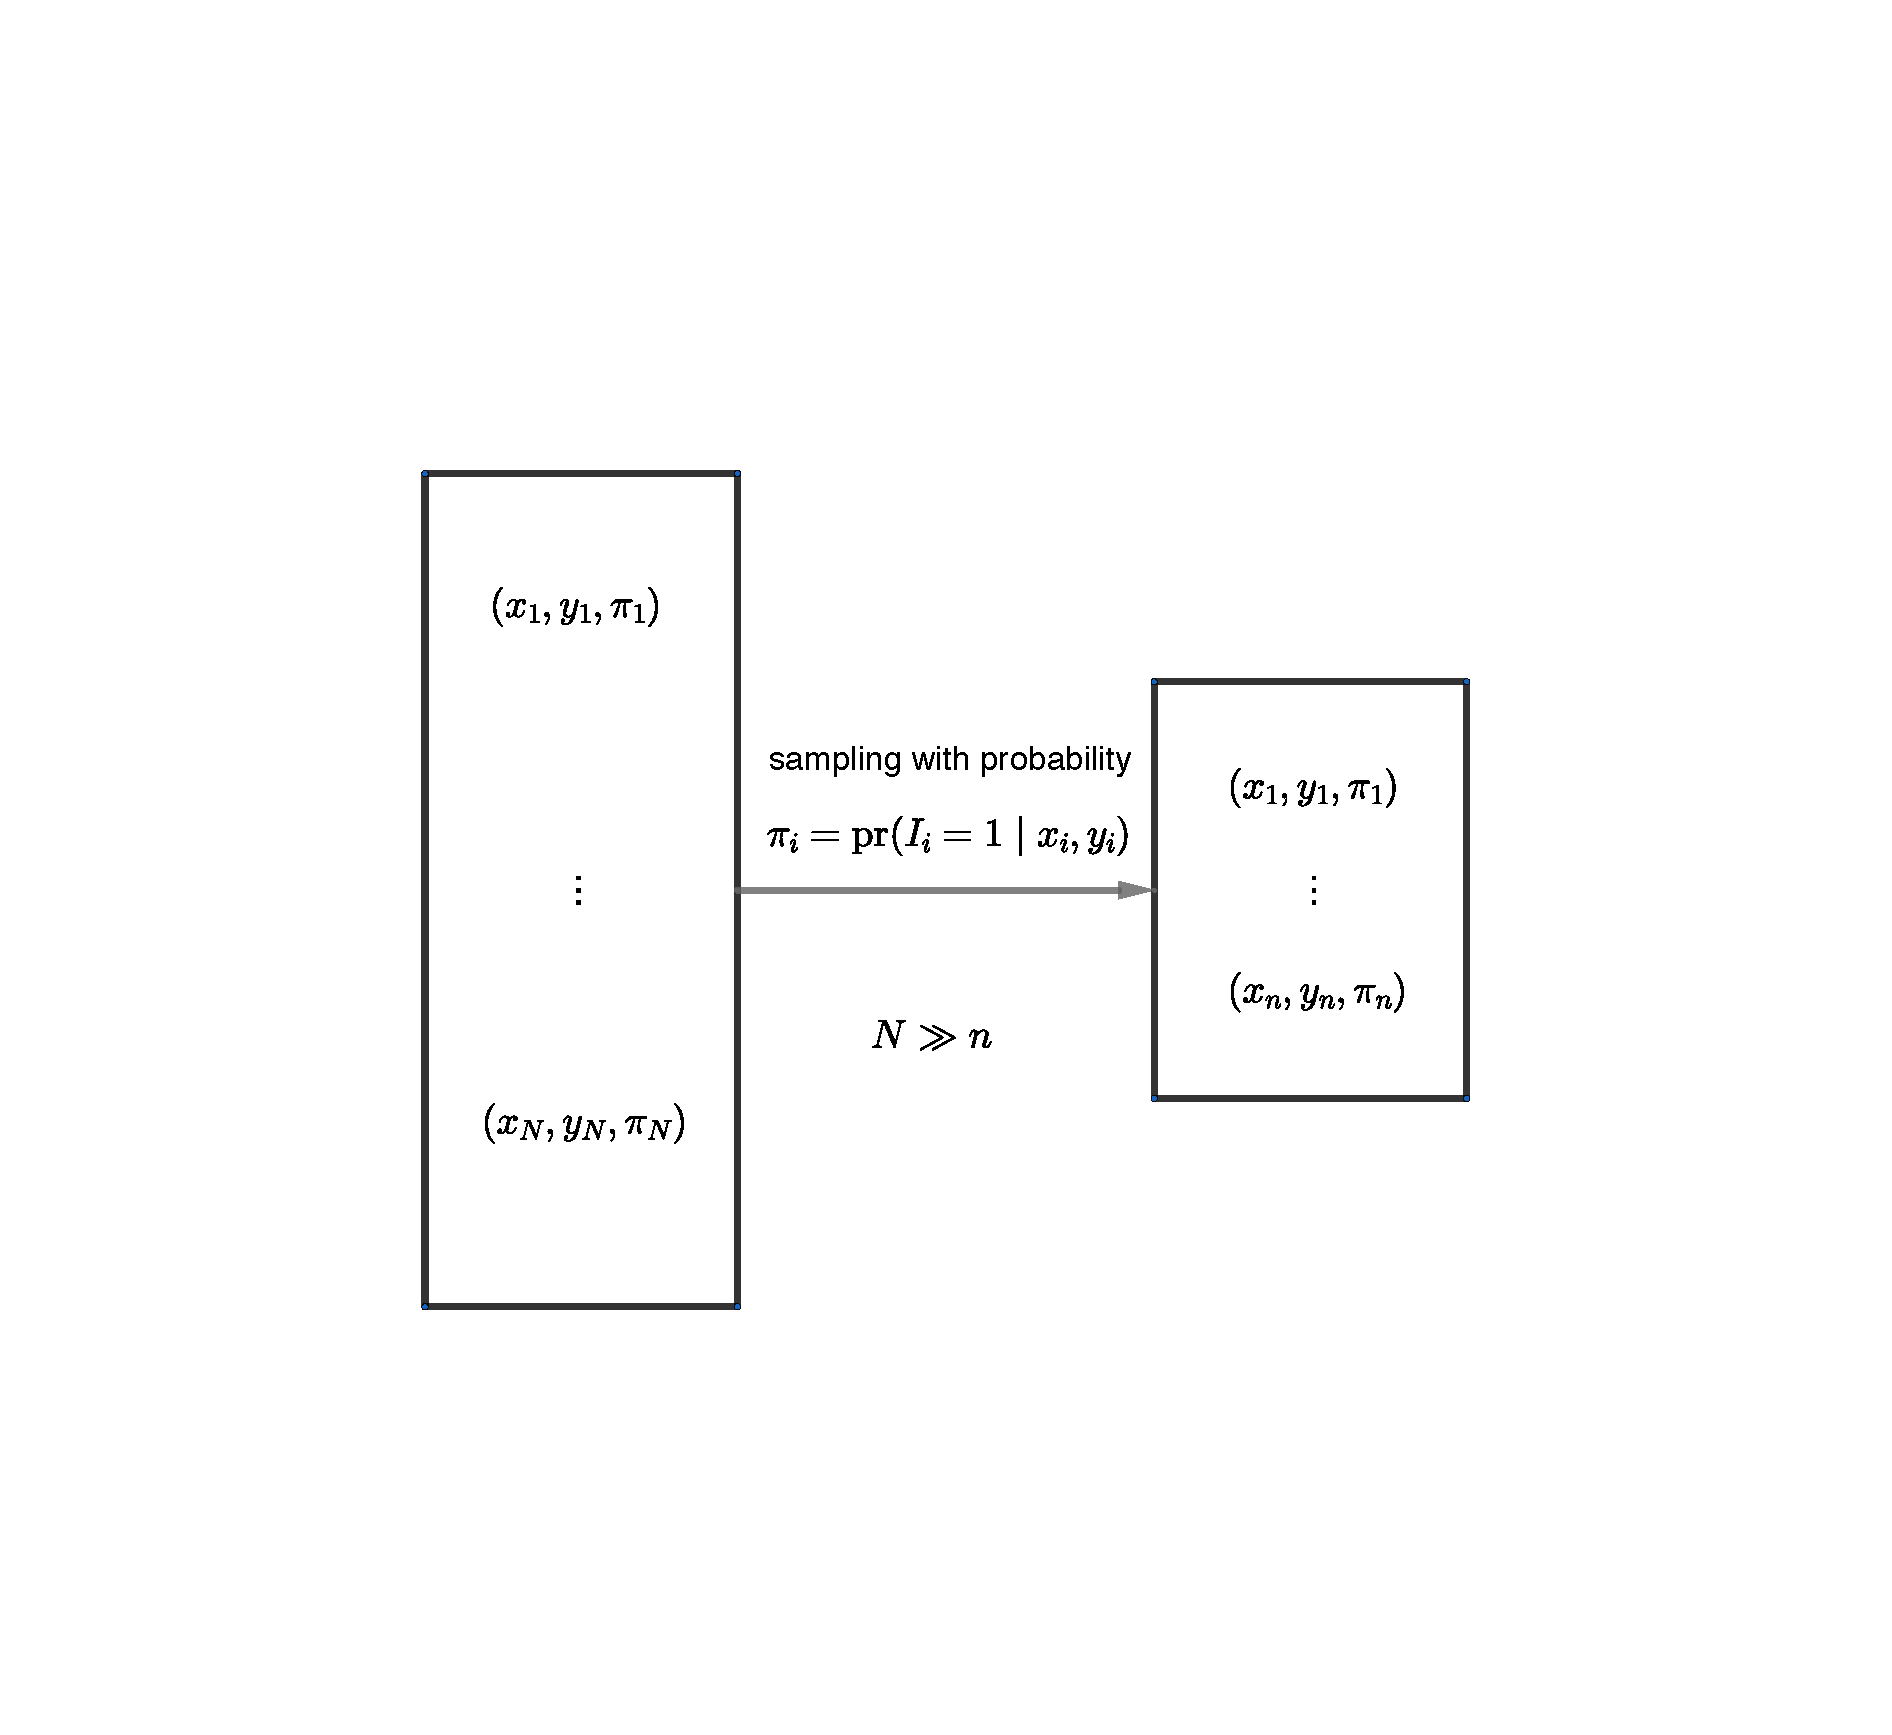
\includegraphics[width = 0.9\textwidth]{figures/surveysamplingplot}
\caption{Survey sampling}
\end{figure}

If we have the large population with size $N$, then the ideal OLS
estimator of the $y_i$'s on the $x_i$'s is
\[
\hat{\beta}_{\text{ideal}}=\left(\sum_{i=1}^{N}x_{i}x_{i}^{\T}\right)^{-1}\sum_{i=1}^{N}x_{i}y_{i}.
\]
However, we do not have all the data points in the large population,
but sample each data point independently with probability
\[
\pi_{i}=\pr(I_{i}=1\mid x_{i},y_{i}),
\]
where $I_{i}$ is a binary indicator for being included in the sample.
Conditioning on $X_N = (x_{i})_{i=1}^N$ and $Y_N = (y_{i})_{i=1}^{N}$, $\hat{\beta}_{\text{ideal}}$ is a fixed number, and an estimator is
the following WLS estimator
\begin{eqnarray*}
\hat{\beta}_{1/\pi} 
&=& \left(\sum_{i=1}^{N}\frac{I_{i}}{\pi_{i}}x_{i}x_{i}^{\T}\right)^{-1}\sum_{i=1}^{N}\frac{I_{i}}{\pi_{i}}x_{i}y_{i}  \\
&=&\left(\sum_{i=1}^{n}\pi_{i}^{-1}x_{i}x_{i}^{\T}\right)^{-1}\sum_{i=1}^{n}\pi_{i}^{-1}x_{i}y_{i},
\end{eqnarray*}
with weights inversely proportional to the sampling probability. This
inverse probability weighting estimator is reasonable because 
\begin{align*}
E\left(\sum_{i=1}^{N}\frac{I_{i}}{\pi_{i}}x_{i}x_{i}^{\T}\mid X_N,Y_N\right) & =\sum_{i=1}^{N}x_{i}x_{i}^{\T},\\
E\left(\sum_{i=1}^{N}\frac{I_{i}}{\pi_{i}}x_{i}y_{i}\mid X_N,Y_N\right) & =\sum_{i=1}^{N}x_{i}y_{i}.
\end{align*}
The inverse probability weighting estimators are called
the Horvitz--Thompson estimators \citep{horvitz1952generalization}, which are the cornerstones of survey sampling. 


Below I use the dataset \ri{census00.dta} to illustrate the use of sampling weight, which is the \ri{perwt} variable. The \ri{R} code is in \ri{code18.4.2.R}.

\begin{lstlisting}
> library(foreign)
> census00 = read.dta("census00.dta")
> ols.fit = lm(logwk ~ age + educ + exper + exper2 + black,
+              data = census00)
> wls.fit = lm(logwk ~ age + educ + exper + exper2 + black,
+              weights = perwt, data = census00)
> compare = cbind(summary(ols.fit)$coef[,1:3], 
+                 summary(wls.fit)$coef[,1:3])
> round(compare, 4)
            Estimate Std. Error t value Estimate Std. Error t value
(Intercept)   5.1667     0.1282    40.3   5.0740     0.1268    40.0
age          -0.0148     0.0067    -2.2  -0.0084     0.0067    -1.3
educ          0.1296     0.0066    19.7   0.1228     0.0065    18.8
exper2        0.0003     0.0001     2.2   0.0002     0.0001     1.3
black        -0.2467     0.0085   -29.2  -0.2574     0.0080   -32.0
\end{lstlisting}

 

\section{Homework problems}
\label{sec::homework-problems}
 
 
\paragraph{A linear algebra fact related to WLS}\label{hw16::linear-algebra-wls} 
 
This problem extends Corollary \ref{corollary::WLS-linear-algebra}.

Show that 
$$
(X^{\T}  \Sigma^{-1}  X) ^{-1} 
\preceq
(X^{\T}  \Omega  X)^{-1}X^{\T}   \Omega  \Sigma   \Omega X(X^{\T}   \Omega  X)^{-1}.
$$
When $ \Omega = \Sigma^{-1}$, the equality holds.  
 

\paragraph{Generalized least squares with a block diagonal covariance}\label{hw16::gls-block-cov}

Partition $X$ and $Y$ into 
$$
X =  \begin{pmatrix}
X_1\\
\vdots \\
X_K
\end{pmatrix},\quad
Y = \begin{pmatrix}
Y_1\\
\vdots\\
Y_K
\end{pmatrix}
$$
corresponding to $\Sigma$ in \eqref{eq::block-diagonal-sigma} such that $X_k  \in \mathbb{R}^{ n_k\times p}$ and $Y_k\in  \mathbb{R}^{n_k}$. Show that the generalized least squares estimator is
$$
\hat{\beta}_\Sigma = \left(\sum_{k=1}^K X_k ^{\T} \Sigma_k^{-1} X_k \right)^{-1} \left( \sum_{k=1}^K X_k ^{\T} \Sigma_k^{-1} Y_k \right).
$$


\paragraph{Univariate WLS}\label{hw16::univariate-wls}


Prove the following Galtonian formula for the univariate WLS:
$$
\min_{a,b}
\sumn w_i (y_i - a - b x_i)^2
$$
has the minimizer
$$
\hat{\beta}_w = \frac{ \sumn w_i(x_i - \bar{x}_w) (y_i - \bar{y}_w) }{ \sumn w_i(x_i - \bar{x}_w)^2  },\quad 
\hat\alpha_w = \bar{y}_w - \hat{\beta}_w  \bar{x}_w
$$
where $ \bar{x}_w = \sumn w_i x_i /  \sumn w_i   $ and $ \bar{y}_w = \sumn w_i y_i /  \sumn w_i $ are the weighted means of the covariate and outcome.



\paragraph{Difference-in-means with weights}\label{hw16::binaryx-wls}

With a binary covariate $x_i$, show that the coefficient of $x_i$ in the WLS of $y_i$ on $(1,x_i)$ with weights $w_i$ $(i=1,\ldots, n)$ equals 
$
\bar{y}_{w,1} - \bar{y}_{w,0},
$
where
$$
\bar{y}_{w,1}   =  \frac{ \sumn w_i x_i y_i  }{ \sumn w_i x_i } ,\quad
\bar{y}_{w,0} =  \frac{ \sumn w_i (1-x_i) y_i  }{ \sumn w_i (1-x_i) }
$$
are the weighted averages of the outcome under treatment and control, respectively. 

Hint: You can use the result in Problem \ref{hw16::univariate-wls}. 

\paragraph{Asymptotic Normality of WLS and robust covariance estimator}

Under the heteroskedastic linear model,  show that $\hat{\beta}_{w}$ is consistent and asymptotically Normal,
and show that $n\hat{V}_{w}$ is consistent for the asymptotic covariance
of $\sqrt{n}(\hat{\beta}_{w}-\beta).$ Specify the regularity conditions. 



\paragraph{WLS in ANOVA}\label{hw16::wls-anova}

This problem extends Problems \ref{hw5:anova-f}  and \ref{hw8::anova-ols-hc02}. 

For units $i=1,\ldots, n$, assume $y_i$ denotes the outcome, $x_i$ denotes the $p$-vector with entries as the dummy variables for a discrete covariate with $p$ levels, $w_i > 0$ denotes a weight, and $\pi_i > 0$ denotes another weight that is a function of $x_i$ only (for example, $\pi_i = n_j/n$ if $x_i = e_j$). Run the following regressions:
\begin{itemize}
\item
WLS of $y_i$ on $x_i$ with weight $w_i$ for $i=1,\ldots, n$ to obtain the coefficient vector $\hat{\beta}$ and EHW covariance matrix $\hat{V}$;
\item
WLS of $y_i$ on $x_i$ with weight $w_i \pi_i$ for $i=1,\ldots, n$ to obtain the coefficient vector $\hat{\beta}'$ and EHW covariance matrix $\hat{V}'$.
\end{itemize}
Show that 
$
\hat{\beta} = \hat{\beta}'  
$ 
with the $j$th entry
$$
\hat\beta_j=\hat\beta_j' = \frac{  \sum_{i: x_i = e_j}  w_i y_i }{  \sum_{i: x_i = e_j}  w_i},
$$
and moreover, $\hat{V} = \hat{V}'$ are diagonal with the $(j,j)$th entry
$$
\hat{V}_{jj} = \hat{V}_{jj}' = \frac{\sum_{i: x_i = e_j}  w_i^2 (y_i - \hat\beta_j)^2 }{ ( \sum_{i: x_i = e_j}  w_i   )^2  }  .
$$

 


\paragraph{An infeasible generalized least squares estimator}

Can we skip Step \ref{enu:fgls-step2} in Section \ref{section::fgls} and directly apply the following
WLS estimator:
\[
\hat{\beta}_{\textsc{igls}}=\left(\sumn\hat{\varepsilon}_{i}^{-2}x_{i}x_{i}^{\T}\right)^{-1}\sumn\hat{\varepsilon}_{i}^{-2}x_{i}y_{i}
\]
with $\hat{\varepsilon}_i = y_i - x_i^{\T} \hat{\beta}$. 
If so, give a theoretical justification; if not, give a counterexample. Evaluate the finite-sample properties of $\hat{\beta}_{\textsc{igls}}$ using simulated data.


\paragraph{FWL theorem in WLS}\label{hw16::fwl-wls}

This problem is an extension of Theorem \ref{thm:fwl}. 

Consider the WLS with an $n\times 1$ vector $Y$, an $n\times k$ matrix $X_1$, an $n\times l$ matrix $X_2$, and weights $w_{i}$'s. 
Show that $\hat{\beta}_{w,2} $ in the long WLS fit
\[
Y=X_{1}\hat{\beta}_{w,1}+X_{2}\hat{\beta}_{w,2}+\hat{\varepsilon}_{w}
\]
equals the coefficient of $\tilde{X}_{w,2}$ in the WLS fit of $\tilde{Y}_{w}$ on  $\tilde{X}_{w,2}$,
%\[
%\hat{\beta}_{w,2} =(\tilde{X}_{w,2}^{\T}\tilde{X}_{w,2})^{-1}\tilde{X}_{w,2}^{\T}\tilde{Y}_{w},
%\]
where $\tilde{X}_{w,2}$ are the residual vectors from the column-wise
WLS of $X_{2}$ on $X_{1}$, and $\tilde{Y}_{w}$ is the residual
vector from the WLS of $Y$ on $X_{1}$. 


\paragraph{The sample version of Cochran's formula in WLS}\label{hw16::wls-sample-cochran-formula}

This problem is an extension of Theorem \ref{thm::cochran-formula}. 


Consider the WLS with an $n\times 1$ vector $Y$, an $n\times k$ matrix $X_1$, an $n\times l$ matrix $X_2$, and weights $w_{i}$'s. 
We can fit the following WLS:
\begin{eqnarray*}
Y &=& X_1 \hat{\beta}_{w,1} + X_2 \hat{\beta}_{w,2}+ \hat{\varepsilon}_{w},\\
Y &=& X_2 \tilde{\beta}_{w,2} + \tilde{\varepsilon}_w ,\\
X_1 &=& X_2 \hat{\delta}_w + \hat{U}_w,
\end{eqnarray*}
where $\hat{\varepsilon}_w, \tilde{\varepsilon}_w , \hat{U}_w$ are the residuals. 
The last WLS fit means the WLS fit of each column of $X_1$ on $X_2$. Similar to Theorem \ref{thm::cochran-formula}, we have 
$$
\tilde{\beta}_{w,2} = \hat{\beta}_{w,2} +  \hat{\delta}_w \hat{\beta}_{w,1}.
$$
Prove this result. 



\paragraph{EHW robust covariance estimator in WLS}\label{hw16::ehw-wls}

We have shown in Section \ref{section::GLS} that the coefficients from WLS are identical to those from OLS with transformed variables.
Further show that the corresponding HC0 version of EHW covariance estimators are
also identical. 

 
 
 \paragraph{Invariance of  covariance estimators in WLS}\label{hw16::invariance-cov-wls}

Problem \ref{hw08::invariance-ehw01234} states the invariance of covariance estimators in OLS. Show that the same result holds for covariance estimators in WLS. 
 
 


\paragraph{Ridge with weights}

Define the ridge regression with weights $w_{i}$'s, and derive the
the formula for the ridge coefficient. 

\paragraph{Coordinate descent algorithm in lasso with weights}

Define the lasso with weights $w_{i}$'s, and give the coordinate
descent algorithm for solving the weighted lasso problem. 



\paragraph{General leave-one-out formula via WLS}
\label{hw16::loo-wls}



With data $(X,Y)$, we can define $\hat{\beta}_{[-i]}(w)$ as the WLS estimator of $Y$ on $X$ with weights $w_{i'} = 1(i' \neq i) + w 1(i'=i)$ for $i' = 1,\ldots, n$, where $ 0\leq w \leq 1$.  It reduces to the OLS estimator $\hat\beta$ when $w=1$ and the leave-one-out OLS estimator $\hat{\beta}_{[-i]}$ when $w=0$. 

Show the general formula 
$$
\hat{\beta}_{[-i]}(w) = \hat{\beta}  - \frac{1-w}{1-(1-w)h_{ii}}  (X^{\T} X)^{-1} x_i \hat{\varepsilon}_i
$$
recalling that $h_{ii}$ is the leverage score and $\hat{\varepsilon}_i$ is the residual of observation $i$. 



Remark: 
Based on the above formula, we can compute the derivative of $\hat{\beta}_{[-i]}(w) $ with respect to $w$:
$$
\frac{ \partial  \hat{\beta}_{[-i]}(w)  }{  \partial  w } = \frac{1}{\{ 1-(1-w)h_{ii} \}^2} (X^{\T} X)^{-1} x_i \hat{\varepsilon}_i,
$$
which reduces to 
$$
\frac{ \partial  \hat{\beta}_{[-i]}(0)  }{  \partial  w } = \frac{1}{( 1-h_{ii} )^2} (X^{\T} X)^{-1} x_i \hat{\varepsilon}_i
$$
at $w=0$ and 
$$
\frac{ \partial  \hat{\beta}_{[-i]}(1)  }{  \partial  w } =  (X^{\T} X)^{-1} x_i \hat{\varepsilon}_i
$$
at $w=1$. 
\citet{pregibon1981logistic} reviewed related formulas for OLS.
\citet{broderick2020automatic} discussed related formulas for general statistical models. 




 
 \paragraph{Hat matrix and leverage score in WLS}
 \label{hw16::hat-matrix-leverage-scores}
 
 
 Based on the WLS estimator $\hat{\beta}_w = (X^{\T}  W X)^{-1} X^{\T} W Y $ with $W = \text{diag}(w_1, \ldots, w_n)$, we have the predicted vector 
 $$
 \hat{Y}_w = X \hat{\beta}_w  =  X (X^{\T}  W X)^{-1} X^{\T} W Y.
 $$
 This motivates the definition of the hat matrix 
 $$
H_w =   X (X^{\T}WX)^{-1} X^{\T}W 
$$
 such that $ \hat{Y}_w = H_w Y$. 
 
First, show the following basic properties of the hat matrix:
$$
WH_w = H_w^{\T} W,\quad X^{\T} W (I_n - H_w) = 0.
$$

Second, prove an extended version of Theorem \ref{thm::leverage-mdist}: with $x_i = (1,x_{i2}^{\T} )^{\T} $, the $(i,i)$th diagonal element of $H_w$ satisfies
$$
h_{w,ii} = \frac{w_i}{  \sum_{i'=1}^n w_{i'} }  (1 + D_{w,i}^2)
$$ 
where 
$$
D_{w,i}^2 =   (x_{i2} - \bar{x}_{w,2})^{\T} S_w^{-1}  (x_{i2} - \bar{x}_{w,2})
$$
with $\bar{x}_{w,2} = \sumn  w_i x_{i2}  / \sumn  w_i $ being the weighted average of $x_{i2}$'s and  $S_w   =   \sumn w_i (x_{i2} - \bar{x}_{w,2})(x_{i2} - \bar{x}_{w,2})^{\T} / \sumn w_i  $ being the corresponding sample covariance matrix. 
 
 



 
 Remark: 
\citet{li2009survey} presented the basic properties of $H_w$ for WLS in the context of survey data. 




\paragraph{Leave-one-out formula for WLS}
\label{hw16::loo-for-wls}


Use the notation in Problem \ref{hw16::hat-matrix-leverage-scores}. 
Let $\hat\beta_w$ be the WLS estimator of $Y$ on $X$ with weights $w_i$'s. Let $\hat{\beta}_{w[-i]}$ be the WLS estimator without using the $i$th observation. Show that 
$$
\hat{\beta}_{w[-i]} = \hat\beta_w - \frac{ w_i }{ 1-h_{w,ii} }  (X^{\T} W X)^{-1} x_i \hat{\varepsilon}_{w,i} .
$$







\paragraph{EHW standard errors in WLS}

Report the EHW standard errors in the examples in Sections \ref{section::fgls}, \ref{sec::regression-aggregateddata}, and \ref{sec::regression-surveydata}. 


 
 
 
\paragraph{Another example of ecological inference}\label{hw16::ecological-regression2}

The \ri{fultongen} dataset in the \ri{ri} package contains aggregated data from 289 precincts in Fulton County, Georgia. The variable \ri{t} represents the fraction voting in 1994 and \ri{x} the fraction in 1992. The variable \ri{n} represents the total number of people. Run ecological regression similar to   Section \ref{sec::regression-aggregateddata}. 



